\section{Machine learning protocols}
\subsection{Apprentissage supervisé}
L'apprentissage supervisé est une technique d'apprentissage \textcolor{blue}{\textbf{automatique}} où l'on cherhcer à produire \textbf{automatiquement des règles} à partir d'une base de données contenant des examples déjà traités. Le but de la méthode est de déterminer une représentation compacte de la base de données par une fonction dite de prédiction associant à une entrée, une sortie.\\
\Exemple: KNN, decision tree, Neural network. \\
\textbf{Application}: reconnaissance d'image, ou plus récemment la suppresion d'objet dans une image(application dans photoshope). 
\begin{figure}[H]
    \centering
    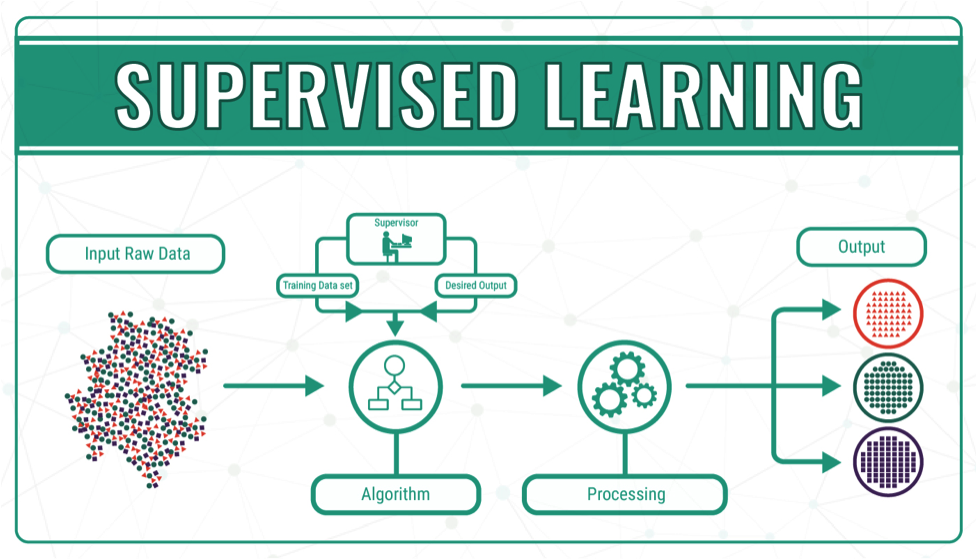
\includegraphics[scale = 0.5]{Question1/supervised-learning.png}
    \caption{}
    \label{fig:my_label}
\end{figure}
\subsection{Apprentissage non-supervisé}
L'apprentissage \textbf{non supervisé} est un problème d'apprentissage automatique. Il s'agit de trouver des stuctures sous-jacentes à partir de donnée \textbf{non} étiquetées. Puisque les données ne sont pas étiquetées, il n'est pas possible d'affecter  au résultat de l'algorithme utilisé un score d'adéquation. Cette absence d'étiquetage(ou d'annotation) est ce qui distingue les taches d'apprentissage non-supervisé des tâches d'apprentissage supervisé.
\begin{figure}[H]
    \centering
    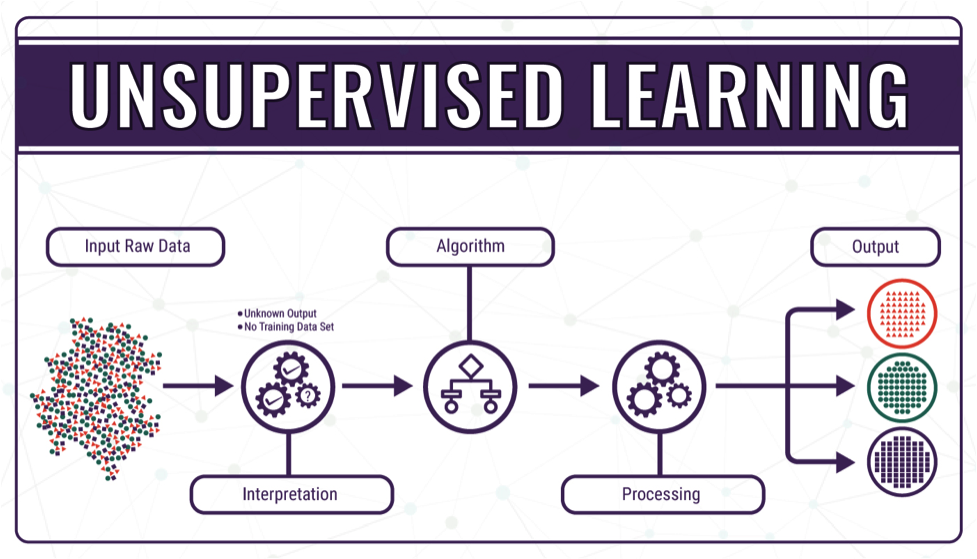
\includegraphics[scale = 0.5]{Question1/unsupervised-learning.png}
    \caption{}
    \label{fig:my_label}
\end{figure}

\subsection{Apprentisage non-supervisé vs. supervisé}
On distingue l'apprentissage supervisé et non supervisé. Dans le permier cas, il s'agit d'apprendre à classer un nouvel individu parmi un ensemble de classes prédéfinies: on connait les classes à priori. Tandis que dans l'apprentissage non supervisé, le nombre et la définition des classes ne sont pas donnés à priori.

\subsection{Apprentissage par renforcement}
L'apprentissagr par renforcement fait référence à une classe de problémes d'apprentissage automatique à partir d'expériences de façons à optimiser une récompense numérique au cours du temps. Un agent autonome, plongé au sein d'un environnement, cherche au travers d'expériences itérés un comportement décisionnel optimal, une politique (fonction) associant sont état courant à l'action à exécuter permettant de maximiser la somme des récompenses au cours du temps.

\begin{figure}[H]
    \centering
    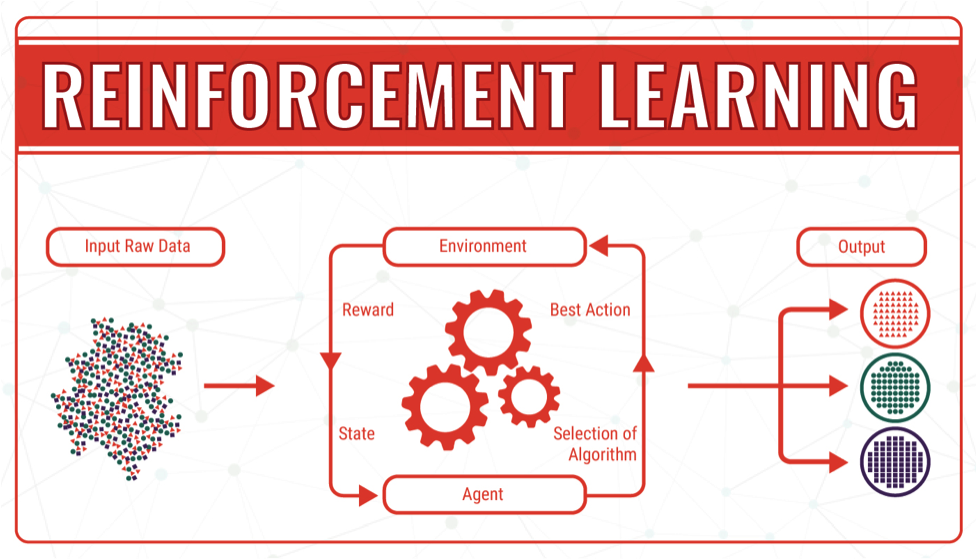
\includegraphics[scale = 0.25]{Question1/reinforcement-learning.png}
    \caption{}
    \label{fig:my_label}
\end{figure}
\subsubsection{Apprentissage en mode hors line (batch)}
\textcolor{red}{\textbf{Il exploite un max la DB}}\\
L'apprentissage en mode hos ligne(ou \textbf{batch}) est un cas particulier du reinforcement learning, qui est une classe de problèmes d'apprentisage dont l'obejectif est de déterminer à partir d'expériences une stratégie (ou politique) permettant à un agent de maximiser une récompense numérique au cours du temps.\\
Dans le cadre de l'apprentissage par renforcement purement hors ligne, l'agent ne peut interagir avec l'environnement: une base d'apprentissage lui est fournie au départ et il l'exploite pour apprendre une politique.\\\\
\textbf{Compément d'information}\\\\
Contrastant avec les algorithmes en-ligne, où l'agent à la possibilité d'interagir comme bon lui semble avec l'environnement, les algorithmes hors-ligne tentent d'exploiter au maximum les exemples d'apprentissage dont ils disposent, sans compter uniquement sur la possibilité d'exploration. Cette approche est donc particulièrement avantageuse quand il n'est pas possible d'effectuer des expériences ou lorsque ces expériences sont coûteuses (casse de matériel possible, obligation d'avoir recours à une assistance humaine pendant les expériences, etc). En général cependant, les techniques d'apprentissage par renforcement batch peuvent être utilisées

\subsubsection{Apprentissage en mode batch vs. apprentissage en mode on-line}
\begin{itemize}
    \item En mode \textbf{batch}, les échantillons sont fournis et calculés ensemble pour former le modèle alors qu'en mode on-line, les échantillons sont données un à un pour mettre à jour le modèle.
    \item E mode \textbf{batch}, les échantillons sont stockés et non le modèle, tandis qu'en mode on-line c'est le modèle qui est stocké et non les échantilons. 
    \item Le mode batch est une approche classique du data-mining alors que le mode \textbf{on-line} est une methode approche pour les systèmes adaptatifs.
\end{itemize}
Les deux mode peuvent êtrre adapté pour répondre à un même problème: pour des échantillons donnée, on peut les exploiter un par un pour obtenir un mode on-line,ainsi que, pour des échantillons donnée un par un on peut les stocker avant de les exploiter tous ensemble.\\
\textbf{Exemple: Reconnaissance de symboles manuscrits}
\\\\
\textbf{Complément d'information}\\\\
L’exploration de données, connue aussi sous l'expression de fouille de données, forage de données, prospection de données, \textbf{data mining}, ou encore extraction de connaissances à partir de données, a pour objet l’extraction d'un savoir ou d'une connaissance à partir de grandes quantités de données, par des méthodes automatiques ou semi-automatiques.
Elle se propose d'utiliser un ensemble d'algorithmes issus de disciplines scientifiques diverses telles que les statistiques, l'intelligence artificielle ou l'informatique, pour construire des modèles à partir des données, c'est-à-dire trouver des structures intéressantes ou des motifs selon des critères fixés au préalable, et d'en extraire un maximum de connaissances.
\subsection{Apprentissage semi-supervisé}
Le but de cet apprentissage est d'exploiter à la fois des données labélisées et celles qui ne le sont pas pour construire de meilleurs modèles que si on n'utilisait qu'un seul typde de données.\\
Différentes approches sont possibles : 
\begin{itemize}
    \item \textbf{SVM} semi-supervisé: énumérer toutes les labelisations possible (pour les données non labélisées), apprendre un SVM pour chacune et ne garder que celle avec la plus grande marge d'erreur. 
    \item Algo basé sur les graphes: Construire un graphe sur base des données des 2 types et apprendre un modèles qui prédit correctement les données et qui lisse le graphe.
\end{itemize}
\textbf{Exemple}: Diagnostique médical par \textbf{SVM}
\subsection{Apprentissage transductif}
Semblable à l'apprentissage supervisé mais on a accès dès le début aux données de test qu'on veut utiliser sans construire de modèle pour calculer les prédictions des données non labélisées.\\
\textbf{Solution simple}: appliquer des techniques d'apprentissage semi-supervisé en utilisant des données de test comme données non labélisées pour obtenir un modèle qui servira à prédire les données de test.
